\section{The Radix-$2^3$ FFT  Algorithm}
\begin{frame}
  \frametitle{\textbf{Table of Contents}}
  \begin{center}
    {\vspace{-1.5cm}\Large \textbf{Sección \thesection}\vspace{0.5cm}}
    \begin{beamercolorbox}[
      sep=8pt,center]{part title}
      \usebeamerfont{part title}
      \textbf{\insertsection}
    \end{beamercolorbox}
  \end{center}
\end{frame}

\begin{frame}
	\frametitle{\textbf{The Radix-$2^3$ FFT  Algorithm}}
	\framesubtitle{\secname : \subsecname}
	\begin{block}{\centering}
		\begin{itemize} %\justifying\footnotesize
			\item The \textit{N}-point DFT of an input sequence $x[n]$ is defined as:

				\begin{equation}
					X[k] = \sum_{n=0}^{N-1} x[n] \dot W_N^{nk}, \quad k=0,1,...,N-1
				\end{equation}
					where $W_N^{nk} = e^{-j\frac{2\pi}{N} nk}$. 
		 	\item Appling a \textit{Divide and Conquer} approach we can calculate the DFT in series of $s=log_\rho N$ stages, where $\rho$ is the base of the 			\textit{radix}. 
		 	
		 	\item In our case, the numeber of stages is:
		 	
		 		\begin{equation}
		 			s = log_2 (128) = 7 
		 		\end{equation}
		     	    	
    	\end{itemize}
    \end{block}
\end{frame}


\begin{frame}
  	\frametitle{\textbf{The Radix-$2^3$ FFT  Algorithm}}
	\framesubtitle{\secname : \subsecname}
	\begin{block}{\centering}
		\begin{itemize} %\justifying\footnotesize		

			\item There are two methods to design FFT algorithms:
				\begin{enumerate}
					\item Decimation In Time (DIT).
					\item Decimation In Frcuency (DIF).
				\end{enumerate}											
				
					
			\item The difference is the instant in which the multiplication by $W_N^\phi$ is accomplished. 
			
  		\end{itemize}

  	\end{block}

    %\vspace{-0.2cm}
    \begin{figure}[h!] \centering
    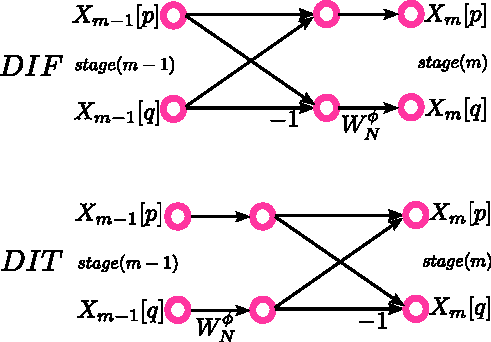
\includegraphics[width=0.45\paperwidth]{./image/DifDit.pdf}
    \caption{\footnotesize Basic butterflies computation in the decimation in time and frequency.}
    \end{figure}

\end{frame}

\begin{frame}
  	\frametitle{\textbf{The Radix-$2^3$ FFT  Algorithm}}
	\framesubtitle{\secname : \subsecname}
	\begin{block}{\centering}
	\begin{itemize}
		\item The input samples in FFT algorithms DIF are 	organized in natural order but its output has not in order.
		\item  The opposite is for DIT. 
		\item Is necessary a circuit for reordering the output data.		 
	\end{itemize}
\end{block}
    \begin{figure}[h!] \centering
    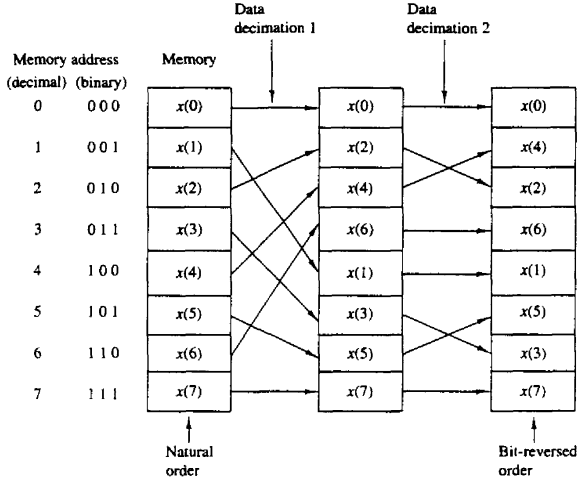
\includegraphics[width=0.4\paperwidth]{./image/dif_order.png}
    \caption{\footnotesize Order of intpus and outputs for DIF FFT.} % Añadir referencia
    \end{figure}
\end{frame}

\begin{frame}
  	\frametitle{\textbf{The Radix-$2^3$ FFT  Algorithm}}
	\framesubtitle{\secname : \subsecname}
	\begin{block}{\centering}
	\begin{itemize}
		\item The fundamental equations for DIF are:
		 
	\end{itemize}			
		
		
	\end{block}
    
    
\end{frame}

\begin{frame}

    \begin{figure}[h!] \centering
    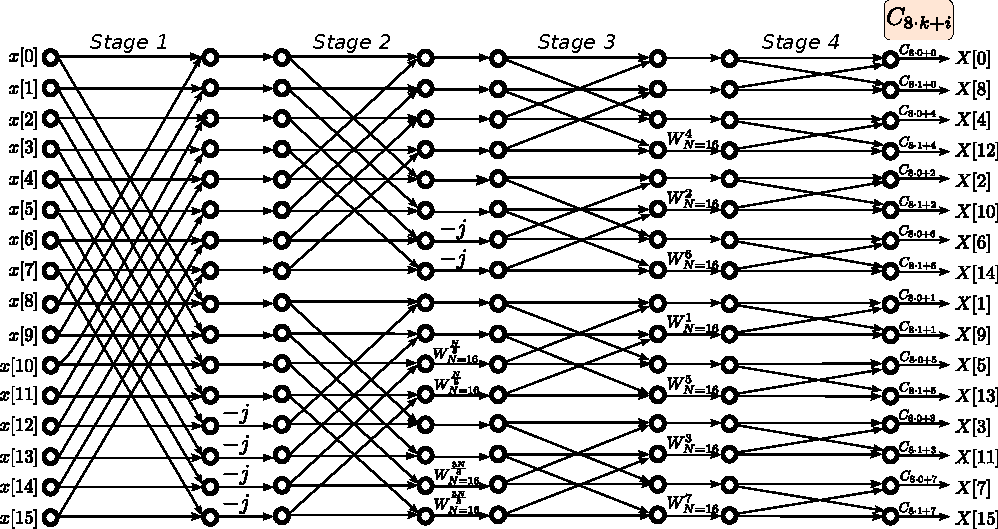
\includegraphics[width=0.7\paperwidth]{./image/16points_con.pdf}
    \caption{\footnotesize Flow graph of a radix-$2^3$ 16-point DIF DFT.}
    \end{figure}
\end{frame}
    
\begin{frame}

    \begin{figure}[h!] \centering
    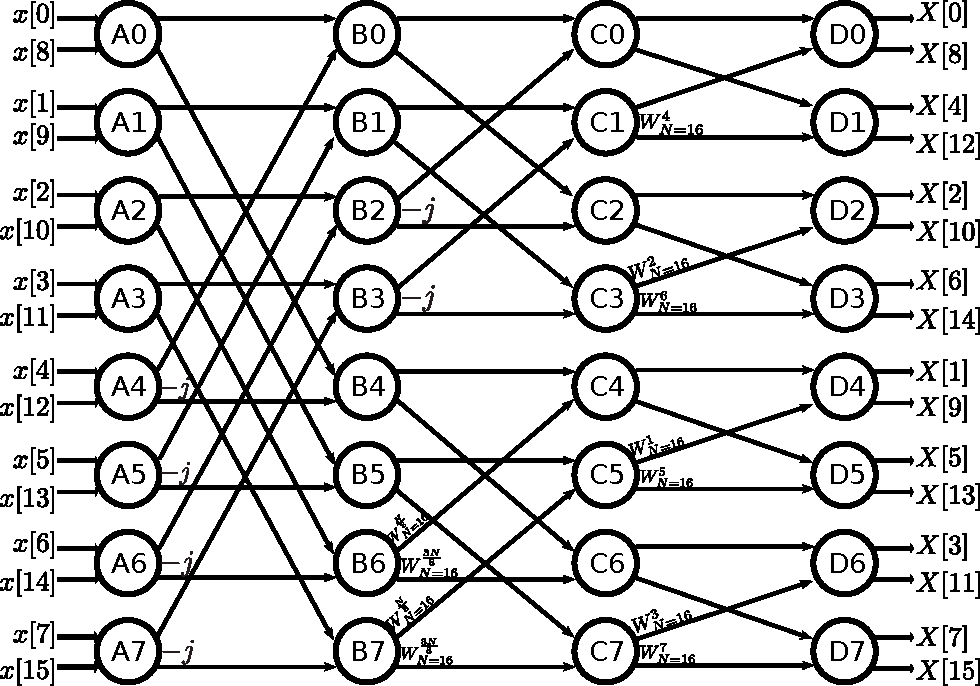
\includegraphics[width=0.5\paperwidth]{./image/16points_dfg.pdf}
    \caption{\footnotesize Data flow graph (DFG) of a radix-$2^3$ 16-point DIF DFT.}
    \end{figure}    
    
\end{frame}